\section{Software: Hawen}
\label{sec:WP1:Hawen:software}

\begin{table}[h!]
    \centering
    { \setlength{\parindent}{0pt}
    \def\arraystretch{1.25}
    \arrayrulecolor{numpexgray}
    {\fontsize{9}{11}\selectfont
    \begin{tabular}{!{\color{numpexgray}\vrule}p{.4\textwidth}!{\color{numpexgray}\vrule}p{.6\textwidth}!{\color{numpexgray}\vrule}}
        \rowcolor{numpexgray}{\rule{0pt}{2.5ex}\color{white}\bf Field} & {\rule{0pt}{2.5ex}\color{white}\bf Details} \\
        \rowcolor{white}\textbf{Consortium} & \begin{tabular}{l}
Inria\\
\end{tabular} \\
        \rowcolor{numpexlightergray}\textbf{Exa-MA Partners} & \begin{tabular}{l}
Inria BXSO\\
\end{tabular} \\
        \rowcolor{white}\textbf{Contact Emails} & \begin{tabular}{l}
florian.faucher@inria.fr\\
\end{tabular} \\
        \rowcolor{numpexlightergray}\textbf{Supported Architectures} & \begin{tabular}{l}
CPU Only\\
\end{tabular} \\
        \rowcolor{white}\textbf{Repository} & \href{https://gitlab.com/ffaucher/hawen}{https://gitlab.com/ffaucher/hawen} \\
        \rowcolor{numpexlightergray}\textbf{License} & \begin{tabular}{l}
OSS:: GPL v*\\
\end{tabular} \\
        \rowcolor{white}\textbf{Bottlenecks roadmap} & \begin{tabular}{l}
B10 - Scientific Productivity\\
B11 - Reproducibility and Replicability of Computation\\
B6 - Data Management\\
B7 - Exascale Algorithms\\
\end{tabular} \\
        \bottomrule
    \end{tabular}
    }}
    \caption{WP1: Hawen Information}
\end{table}

\subsection{Software Overview}
\label{sec:WP1:Hawen:summary}

\hawen~uses the Hybridizable discontinuous Galerkin method (HDG) 
for the discretization of the time-harmonic wave problems such 
as \cref{eq:hawen:viscoacoustic,eq:hawen:viscoelastic}.
The method relies on a static condensation of DG method, and we 
refer to, e.g. \cite{Faucher2020adjoint,pham_numerical_2024} 
and the references therein regarding implementation in acoustics and 
elasticity, respectively.
The specificity of the HDG method is to assemble a global linear system 
only in terms of the degrees of freedom (dofs) on the faces of the discretized 
mesh cells. By avoiding the interior dofs, it allows to reduce the computational
cost by reducing the size of subsequent linear system, e.g. \cite{Faucher2020adjoint}.
However, this benefit is only obtained for sufficiently high degrees of 
polynomials, hence requiring robust quadrature method and flexible model representation
on the mesh.
\hawen~uses $p$-adaptivity to adapt the order of the polynomials on each cell
depending on the wavelength.



In~\cref{tab:WP1:Hawen:features} we provide a summary of the software features relevant to the work package which are briefly discussed.

\begin{table}[h!]
    \centering
    { 
        \setlength{\parindent}{0pt}
        \def\arraystretch{1.25}
        \arrayrulecolor{numpexgray}
        {
            \fontsize{9}{11}\selectfont
            \begin{tabular}{!{\color{numpexgray}\vrule}p{.25\linewidth}!{\color{numpexgray}\vrule}p{.6885\linewidth}!{\color{numpexgray}\vrule}}
    
    \rowcolor{numpexgray}{\rule{0pt}{2.5ex}\color{white}\bf Features} &  {\rule{0pt}{2.5ex}\color{white}\bf Short Description }\\ 
    
\rowcolor{white}    dG/hdG & \hawen~uses the HDG method for the discretization, it allows
                             for local $p-$adaptivity, such that each cell of the discretized
                             domain can use a different polynomial orders.
                             \hawen~solves for 1D, 2D and 3D problems using unstructured 
                             simplex meshes.\\
\rowcolor{numpexlightergray}    multiphysics coupling & provide short description here \\
\end{tabular}
        }
    }
    \caption{WP1: Hawen Features}
    \label{tab:WP1:Hawen:features}
\end{table}


\subsection{Parallel Capabilities}
\label{sec:WP1:Hawen:performances}

\hawen~uses MPI and OpenMP parallelism. The HDG method is particularly 
appropriate for parallelism (as other methods in the DG family), such 
that each cell of the mesh can be treated independently in parallel. 
\hawen~has been used on several supercomputers, including GENCI Adastra
with Genoa partition for CPUs parallelism.
\hawen is linked with MUMPS library, which is a multifrontal direct solver 
for sparse linear systems. 

%\begin{itemize}
%    \item describe the parallel programming  environment : MPI, OpenMP, CUDA, OpenACC, etc.
%    \item describe the parallel computation environment: type of architecture and super computer used.
%    \item describe the parallel capabilities of the software
%    \item \textbf{Scalability:} Describe the general scalability properties of the software
%    \item \textbf{Integration with Other Systems:} Describe how the software integrates with other numerical libraries in the Exa-MA framework.
%\end{itemize}


\subsection{Initial Performance Metrics}
\label{sec:WP1:Hawen:metrics}

This section provides a summary of initial performance benchmarks performed in the context of WP1. It ensures reproducibility by detailing input/output datasets, benchmarking tools, and the results. All data should be publicly available, ideally with a DOI for future reference.

\begin{itemize}
    \item \textbf{Overall Performance:} Summarize the software's computational performance, energy efficiency, and scalability results across different architectures (e.g., CPU, GPU, hybrid systems).
    \item \textbf{Input/Output Dataset:} Provide a detailed description of the dataset used for the benchmark, including:
        \begin{itemize}
            \item Input dataset size, structure, and format (e.g., CSV, HDF5, NetCDF).
            \item Output dataset format and key results.
            \item Location of the dataset (e.g., GitHub repository, institutional repository, or open access platform).
            \item DOI or permanent link for accessing the dataset.
        \end{itemize}
    \item \textbf{open-data Access:} Indicate whether the datasets used for the benchmark are open access, and provide a DOI or a direct link for download. Where applicable, highlight any licensing constraints.
    \item \textbf{Challenges:} Identify any significant bottlenecks or challenges observed during the benchmarking process, including data handling and computational performance.
    \item \textbf{Future Improvements:} Outline areas for optimization, including dataset handling, memory usage, or algorithmic efficiency, to address identified challenges.
\end{itemize}

\subsubsection{Benchmark \#1: Visco-acoustic time-harmonic wave propagation}

\paragraph{Description}
This benchmark considers the propagation of time-harmonic waves in a large-scale
geophysical configuration. We use the model SEAM for this benchmark, which is of
size \num{35}$\times$\num{45}$\times$\num{35}\si{\km\cubed}.  
It gives us the wave-speed and density models, respectively $\sqrt{\kappa/\rho}$ 
and $\rho$ to solve the acoustic wave problem \cref{eq:hawen:viscoacoustic}.
We illustrate the wave-speed model in \cref{figure:hawen:seam-model}.
This model is challenging as it is relatively large (depending on the frequency
we simulate, see below), and includes high-contrast objects. 
For instance, the maximal value of the wave-speed is about 2.5 times higher than
the minimal value, and an object of high contrast has to be carefully discretized.


The objective is to evaluate the performance when we increase the simulation frequency,
to see the maximal frequency attainable at a reasonable cost with \hawen.
Low frequency typically costs less as the wavelength is larger, and the discretization 
can be relaxed (in terms of number of cells in the mesh and/or polynomial orders).
However, when increasing the frequency, the computational cost increases, and this 
progression of cost vs. frequency will be investigated.

Another objective is to design the most efficient setup for the HDG discretization 
of \hawen. In particular, it is known that HDG is more efficient for high order 
polynomials and this aspect must be enforced for efficient simulations. This benchmark
relies onto CPU parallelism.


\paragraph{Benchmarking Tools Used}
To evaluate the performance of the simulations, we will use the memory consumption, 
which will be separated into the one used at the level of the linear algebra (with 
MUMPS) and the other operations (e.g., matrix storage). 
We also evaluate the execution time, with a similar separation to evaluate the 
performance of the computational blocs separately.
For the linear algebra operations with MUMPS, we will also investigate the number
of flops required to factorize the matrix.

\paragraph{Input/Output Dataset Description} The input correspond to the 
physical models that feed the wave equation, such as the wave-speed illustrated
in \cref{figure:hawen:seam-model}. These are available via the SEAM 
corporation\footnote{\url{https://wiki.seg.org/wiki/SEAM}}.

\paragraph{Results Summary}
We will provide the statistics for the computations with frequency, and 
the comparison of HDG discretization (different meshes and polynomial orders)
to identify the best options.

\paragraph{Challenges Identified} 
There are two main challenges, first the memory footprint of the matrix factorization,
second the efficient high-order polynomials to be used with HDG method to maximize its
efficiency.


%
%\begin{itemize}
%    \item \textbf{Description:} Briefly describe the benchmark case, including the problem size, target architecture (e.g., CPU, GPU), and the input data. Mention the specific goals of the benchmark (e.g., testing scalability, energy efficiency).
%    \item \textbf{Benchmarking Tools Used:} List the tools used for performance analysis, such as Extrae, Score-P, TAU, Vampir, or Nsight, and specify what metrics were measured (e.g., execution time, FLOPS, energy consumption).
%    \item \textbf{Input/Output Dataset Description:}
%        \begin{itemize}
%            \item \textbf{Input Data:} Describe the input dataset (size, format, data type) and provide a DOI or link to access it.
%            \item \textbf{Output Data:} Specify the structure of the results (e.g., memory usage, runtime logs) and how they can be accessed or replicated.
%            \item \textbf{Data Repository:} Indicate where the data is stored (e.g., Zenodo, institutional repository) and provide a DOI or URL for accessing the data.
%        \end{itemize}
%    \item \textbf{Results Summary:} Include a summary of key metrics (execution time, memory usage, FLOPS) and their comparison across architectures (e.g., CPU, GPU).
%    \item \textbf{Challenges Identified:} Describe any bottlenecks encountered (e.g., memory usage, parallelization inefficiencies) and how they impacted the benchmark.
%\end{itemize}

% ----------------------
\begin{figure}[ht!]\centering
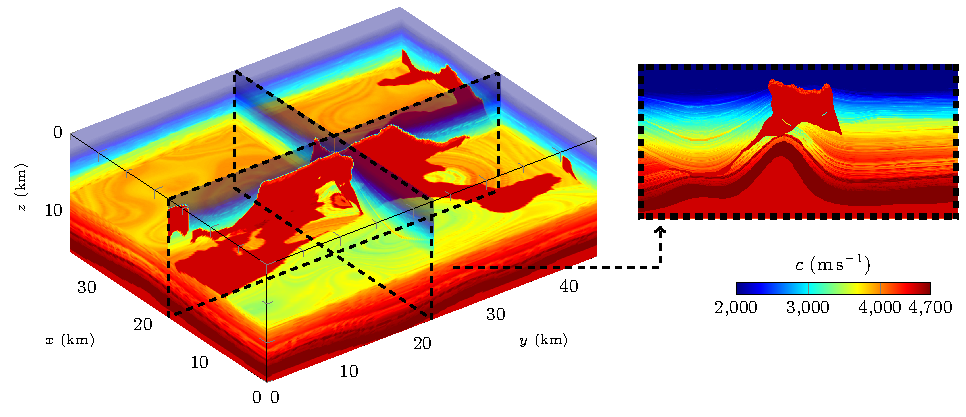
\includegraphics[scale=0.65]{graphics/hawen/skeleton_3D_seam}
\caption{SEAM wave-speed model of size \num{35}$\times$\num{45}$\times$\num{35}\si{\km\cubed} 
         used for the benchmarks.}
\label{figure:hawen:seam-model}
\end{figure}
% ----------------------


\subsubsection{Benchmark \#2: Visco-elastic time-harmonic wave propagation}

The second benchmark is the continuation of the previous one where, instead 
of considering the acoustic problem \cref{eq:hawen:viscoacoustic}, we now
solve the viscoelastic problem with equation~\cref{eq:hawen:viscoelastic}.
Elasticity is computationally much more demanding as, instead of working with
a scalar unknown as in the acoustic case, we now have a vector unknown. 
The configuration of this setup is the same as above, and we also wish to 
compare the performance between acoustic and elastic wave propagation. 
For instance, we wish to identify, for a given computational cost, what 
is the maximal frequency attainable in elastic wave propagation compared to
the acoustic case.
The strategy for the benchmark is the same above, emphasising the use of 
high-order polynomials for HDG in \hawen.


\subsection{12-Month Roadmap}
\label{sec:WP1:Hawen:roadmap}



We wish to improve input/output data management by including more options 
to save the results of \hawen, for instance this can include the hdf5 format
which is not allowed currently.
In addition, the configuration of the benchmark and the results obtained will 
be made available in open-access for reproducibility.
%In this section, describe the roadmap for improving benchmarks and addressing the challenges identified. This should include:
%\begin{itemize}
%    \item \textbf{Data Improvements:} Plans for improving input/output data management, including making datasets more accessible and ensuring reproducibility through open-data initiatives.
%    \item \textbf{Methodology Application:} Implementation of the benchmarking methodology proposed in this deliverable to streamline reproducibility and dataset management.
%    \item \textbf{Results Retention:} Plans to maintain benchmark results in a publicly accessible repository with appropriate metadata and documentation, ensuring long-term usability.
%\end{itemize}
In~\cref{tab:WP1:Hawen:bottlenecks}, we briefly discuss the bottleneck roadmap associated to the software and relevant to the work package.

\begin{table}[h!]
    \centering
    
    

    \centering
    { 
        \setlength{\parindent}{0pt}
        \def\arraystretch{1.25}
        \arrayrulecolor{numpexgray}
        {
            \fontsize{9}{11}\selectfont
            \begin{tabular}{!{\color{numpexgray}\vrule}p{.25\linewidth}!{\color{numpexgray}\vrule}p{.6885\linewidth}!{\color{numpexgray}\vrule}}
    
    \rowcolor{numpexgray}{\rule{0pt}{2.5ex}\color{white}\bf Bottlenecks} &  {\rule{0pt}{2.5ex}\color{white}\bf Short Description }\\ 
    
\rowcolor{white}    B10 - Scientific Productivity & provide short description here \\
\rowcolor{numpexlightergray}    B11 - Reproducibility and Replicability of Computation & provide short description here \\
\rowcolor{white}    B6 - Data Management & provide short description here \\
\rowcolor{numpexlightergray}    B7 - Exascale Algorithms & provide short description here \\
\end{tabular}
        }
    }
    \caption{WP1: Hawen plan with Respect to Relevant Bottlenecks}
    \label{tab:WP1:Hawen:bottlenecks}
\end{table}
